\section{Traditional Breast Cancer Diagnosis Methods}
Trained pathologists diagnose breast cancer with specific facilities and equipment[ris wala]. The traditional clinical techniques used to classify breast cancer involve microarray, biopsy and cytology\citep{articlediagnosi}. 
The grading system proposed by the Dept of pathology across multiple universities based in India also suggests that a combination of clinical investigation, mammography and non-invasive methods can detect 99\% of cancers.
However, cytology is the specific diagnosis method that requires microscopic analysis of the specimens to differentiate between the malignant and benign tumours from the cytological images\citep{articlediagnosi}. 
The technique is used in binary cancer classification based on cytological images.

\section{Artificial Neural Networks}

\begin{center}
    \begin{figure}[htp]
        \centering
        \begin{tikzpicture}[
        plain/.style={
          draw=none,
          fill=none,
          },
        dot/.style={draw,shape=circle,minimum size=3pt,inner sep=0,fill=black
          },
        net/.style={
          matrix of nodes,
          nodes={
            draw,
            circle,
            inner sep=8.5pt
            },
          nodes in empty cells,
          column sep=0.6cm,
          row sep=-11pt
          },
        >=latex
        ]
        \matrix[net] (mat)
        {
        |[plain]| \parbox{1cm}{\centering Input\\layer} 
                  & |[plain]| \parbox{1cm}{\centering Hidden\\layer} 
                               & |[plain]| \parbox{1cm}{\centering Output\\layer} \\
                  & |[plain]|                 \\
        |[plain]| &            & |[plain]|    \\
                  & |[plain]|  &              \\
        |[plain]| & |[dot]|                   \\
                  & |[plain]|  & |[dot]|      \\
        |[plain]| & |[dot]|    & |[plain]|    \\
        |[dot]|   & |[plain]|  & |[dot]|      \\
        |[dot]|   & |[dot]|    & |[plain]|    \\
        |[dot]|   & |[plain]|  &              \\
        |[plain]| &            & |[plain]|    \\
                  & |[plain]|                 \\
        };
        \foreach \ai/\mi in {2/I1,4/I2,6/I3,12/In}
          \draw[<-] (mat-\ai-1) -- node[above] {\mi} +(-1cm,0);
        \foreach \ai in {2,4,6,12}
        {\foreach \aii/\mii in {3/H1,11/Hn}
          \draw[->] (mat-\ai-1) -- (mat-\aii-2) node[yshift=0.6cm] {\mii};
        }
        \foreach \ai in {3,11}
        {  \draw[->] (mat-\ai-2) -- (mat-4-3);
          \draw[->] (mat-4-3) -- node[above] {O1} +(1cm,0);}
        \foreach \ai in {3,11}
        {  \draw[->] (mat-\ai-2) -- (mat-10-3);
          \draw[->] (mat-10-3) -- node[above] {On} +(1cm,0);}
        \end{tikzpicture}
        
        \caption{Multi Layered Neural Network diagram.}
        \caption{Drawing Credits: https://newbedev.com/drawing-neural-network-with-tikz}
        \label{fig_m_3}
        \end{figure}
\end{center}


There are various solutions for the classification problem some of them includes training the convolutional network, the section provides background on the artificial neural networks. The artificial neural networks also known as the ANN are 
biological inspired interconnected networks of neurons \citep{AGATONOVICKUSTRIN2000717}. 
The deep neural networks are based on the  perceptron based learning 
proposed by Frank Rosenblatt\citep{perceptron_learning}. The perceptron model had the limitation of only being applied to the linearly separable functions and therefore the deep neural networks were introduced\citep{perceptron_learning}
The neural networks are typically assigned with the weights at each layer, which are fine-tuned in the training phase of the model in order to minimize the cost function, which reflects the difference between 
the predicted classification value and actual value, the objective is to minimize the objective function also known as the cost function by updating the weights throughout the network\citep{perceptron_learning}
The typical neural network has various layers and each layer contains the set of neurons with the weights associated with the neurons from the various layers, the first layer of the network is known as the input layer, followed 
by various hidden layers and at last the output layer as shown in the fig[2.1] \citep{AGATONOVICKUSTRIN2000717}.

\subsection{Convolutional Neural Network }
\begin{center}
    \begin{figure}[!htp]
        \centering
        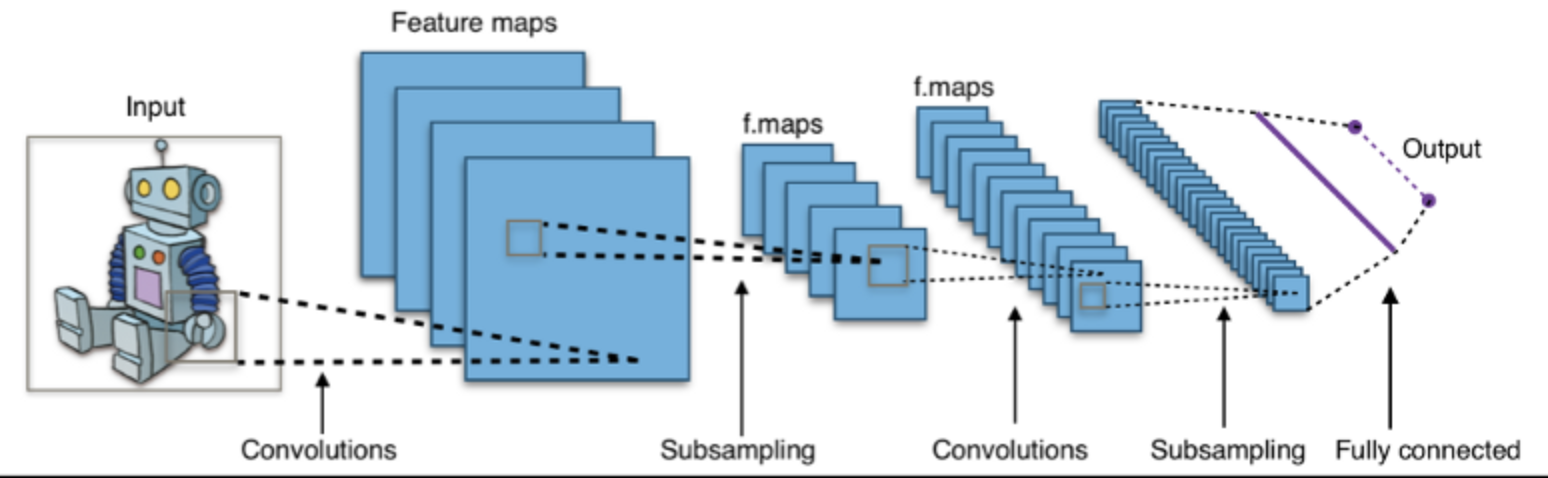
\includegraphics[keepaspectratio=true, scale=0.55]{assets/cnn-model_sample}
        \caption{Convolutional Neural Networks}
        \caption{Image Credits: $en.wikipedia.org/wiki/Convolutional_neural_network$}
        \label{fig:colorchannelseperation}
    \end{figure}
    
\end{center}

CNN are the special kinds of the neural networks which are generally used for the image recognition and image processing tasks[78]. The model intakes the image in the form of the pixels array with separate rgb channels and in order to extract the features from the images, the image kernels or convolutions are performed on the images to extract the feature maps[78]. Furthermore, the feature maps extracted from the convolutional layers are passed to the polling layer which downsamples the features resulting in the dimensionality reduction to the most prominent features in the images which are passed through the respective activation function chosen for the investigation. At the later layers, the feature maps are flattened and passed to the fully connected neural network explained in the previous[78]. 

\section{Transfer Learning}

\subsection{Why transfer learning is required}
The difficulty with training the ANN / CNN is that it is highly reliant on the huge dataset with high accuracy and precision for the training and validation phase,
which in real life scenario is difficult to obtain and cost ineffective solution. The convolutional neural networks also require hyper-parameter tuning.
in order to avoid the overfitting problem in the optimisation step of network training which is a time consuming process\citep{seldon}. 

\subsection{ How transfer-learning operates}

Transfer learning reuses experiential learning from pre-trained models which were trained to 
perform classification on similar dataset[99]. The pre-trained model's weights are used in the fine-tuning phase of the new model 
and therefore, it reduces the need for huge amounts of data to train the networks from scratch\citep{seldon}. 